% -----------------------------------------------
% Template for ISMIR Papers
% 2016 version, based on previous ISMIR templates

% Requirements :
% * 6+1 page length maximum
% * 2MB maximum file size
% * Copyright note must appear in the bottom left corner of first page
% (see conference website for additional details)
% -----------------------------------------------

\documentclass{article}
\usepackage{ismir,amsmath,cite}
\usepackage{url}
\usepackage{cleveref}
\usepackage{graphicx}
\usepackage{color}
% \usepackage{hyperref}
\graphicspath{{figs/}}
\usepackage{booktabs}

\def\eg{\emph{e.g.\/}}
\def\ie{\emph{i.e.\/}}
\def\etc{\emph{etc.\/}}
\def\etal{\emph{et al.\/}}


% Title.
% ------
\title{A Plan for Sustainable MIR Evaluation}

% Note: Please do NOT use \thanks or a \footnote in any of the author markup

% Single address
% To use with only one author or several with the same address
% ---------------
%\oneauthor
% {Names should be omitted for double-blind reviewing}
% {Affiliations should be omitted for double-blind reviewing}

% Two addresses
% --------------
%\twoauthors
%  {First author} {School \\ Department}
%  {Second author} {Company \\ Address}

%% To make customize author list in Creative Common license, uncomment and customize the next line
%  \def\authorname{First Author, Second Author}


% Three addresses
% --------------
\threeauthors
  {First Author} {Affiliation1 \\ {\tt author1@ismir.edu}}
  {Second Author} {\bf Retain these fake authors in\\\bf submission to preserve the formatting}
  {Third Author} {Affiliation3 \\ {\tt author3@ismir.edu}}

%% To make customize author list in Creative Common license, uncomment and customize the next line
%  \def\authorname{First Author, Second Author, Third Author}

% Four or more addresses
% OR alternative format for large number of co-authors
% ------------
%\multauthor
%{First author$^1$ \hspace{1cm} Second author$^1$ \hspace{1cm} Third author$^2$} { \bfseries{Fourth author$^3$ \hspace{1cm} Fifth author$^2$ \hspace{1cm} Sixth author$^1$}\\
%  $^1$ Department of Computer Science, University , Country\\
%$^2$ International Laboratories, City, Country\\
%$^3$  Company, Address\\
%{\tt\small CorrespondenceAuthor@ismir.edu, PossibleOtherAuthor@ismir.edu}
%}
%\def\authorname{First author, Second author, Third author, Fourth author, Fifth author, Sixth author}


\sloppy % please retain sloppy command for improved formatting

\begin{document}

%
\maketitle
%
\begin{abstract}
% MIREX is great!
The Music Information Retrieval Evaluation eXchange (MIREX) is a valuable community service, having established standard datasets, metrics, baselines, methodologies, and infrastructure for comparing MIR methods.
% ...but we can't keep this up. sad!
While MIREX has managed to successfully maintain operations for over a decade, its long-term sustainability is at risk without considerable ongoing financial support.
% Main problem: the expenditure of effort is intrinsically unsustainable.
The imposed constraint that input data cannot be made freely available to participants
necessitates that all algorithms run on centralized computational resources, which are
administered by a limited number of people.
This incurs an approximately linear cost with the number of submissions, exacting
significant tolls on both human and financial resources, such that the current paradigm
becomes \emph{less} tenable as participation increases.
% what's worse, data depletion is unavoidable.
%Meanwhile, successive benchmarking iterations unavoidably deplete the value of annotated data for evaluation purposes, and is a resource that requires constant replenishing. % replacement?
% Main idea: Use one problem to solve the other.
To alleviate the recurring costs of future evaluation campaigns, we propose a distributed,
community-centric paradigm for system evaluation, built upon the principles of openness,
transparency, reproducibility, and incremental evaluation.
%where users contribute annotations over publicly available audio content in order to participate.
% Benefits: sustainability, scalability,
%In this document, we outline the goals, benefits, and limitations of such an approach.
%describe an alternative framework
We argue that this proposal has the potential to reduce operating costs to sustainable
levels.
Moreover, the proposed paradigm would improve scalability, and eventually result in the
release of large, open datasets for improving both MIR techniques and evaluation methods.

\end{abstract}


\section{Introduction}
\label{sec:intro}
% TODO(ejhumphrey|bmcfee)

MIREX has run for several years, and serves a valuable purpose for the community.
It also has a few drawbacks and problems of sustainability.
This document will lay out the goals, benefits, and limitations of MIREX.
We'll then propose an alternative system which should be more sustainable.

% These are rough guesses. @bmcfee halp
The goals of this proposal are threefold:
one, to eventually achieve consensus in the community about how to best proceed with evaluation;
two, establish a feasible plan that is maintainable with minimal resources;
and three, begin to make inroads toward adoption.

\section{MIREX}

% History
The Music Information Retrieval eXcahnge (MIREX) is a framework for the community driven evaluation of MIR algorithms~\cite{downie2008music, downie2010music}.
The annual tradition of MIREX was established early in the lifetime of ISMIR, drawing inspiration from TREC in text IR~\cite{TRECPaperQuestionmark}.
Thanks in large part to the vision of MIR pioneers, the first official iteration took place at ISMIR 2005 after much preliminary work, including a trial run the year prior called the Audio Description Contest (ADC).
The practicalities of MIREX are hosted by the IMIRSEL group at UIUC, and the organization has successfully earned multiple grants to jumpstart the evaluation effort at ISMIR.

% How does this work in practice
At a high level, the typical MIREX paradigm operates as follows:

\begin{enumerate}
\item Identify some task of interest, such as automatic chord estimation.
\item Arrive at a problem formulation and metrics, either in the due course of graduate work or with fellow researchers in the community.
\item Build a corpus of data, with human-annotated ``ground-truth'' annotations for said task.
\item Release a subset of the data for development purposes; retain the rest as private data for evaluation.
\item Invite participants to submit algorithms, which are executed on a private server.
\item Evaluate predicted outputs against reference annotations or human judgments.
\item Repeat steps 5-6 annually. Intermittently repeat step 3, as needed.
\end{enumerate}

% Algorithm-to-data goes astray.
Importantly, this approach differs from TREC-style evaluation by operating in an ``algorithm-to-data'' model, where facilitators oversee the application of code submissions to privately held data, rather than participants submitting predictions over a freely available dataset.
The rationale for this decision is understandable.
In contrast to other machine perception domains, such as natural language processing, speech recognition, or computer vision, intellectual property and copyright law imposes stiff penalties on the illegal distribution of recorded music.
Due to a history of litigation from the Recording Industry Artists of America (RIAA), there is a pervasive sense of fear in the MIR community that sharing audio data would almost certainly result in crippling lawsuits~\cite{downie2008music}.

\begin{figure}[!t]
 \centerline{
 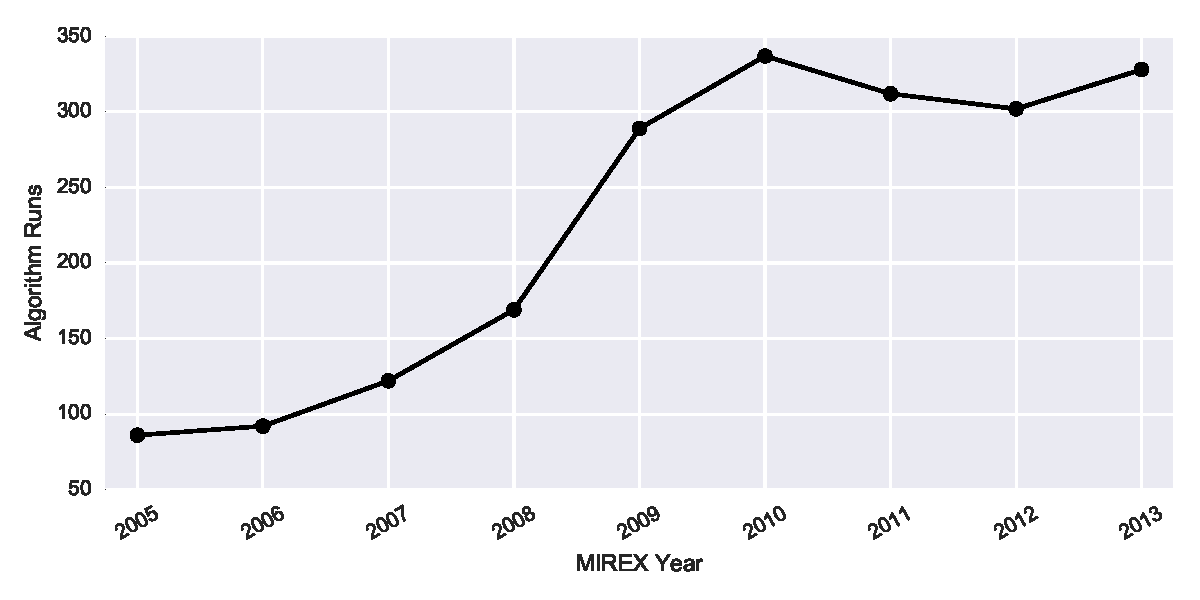
\includegraphics[width=\columnwidth]{mirex_runs.pdf}}
 \caption{Number of algorithms run at MIREX over the course of a almost a decade.}
 \label{fig:system_eval}
\end{figure}

% Deficiencies
% Operating costs are significant
However, experience with MIREX over the last decade has demonstrated that the decision to bring algorithms to data comes with fundamental limitations.
First, as a matter of practicality, doing so incurs remarkably steep costs the community cannot hope to support indefinitely.
Running hundreds of research algorithms demands state of the art technology, and adequate compute cycles must either rented or purchased outright to achieve this.
More often than not, these algorithms are research prototypes, and are seldom optimized for efficiency or ease-of-use.
While task-dependent runtime limits are placed on algorithm execution (between 6 and 72 hours), MIREX is responsible for months to years of compute time annually.
% EJH: I want to mention this, but it really throws off the rhythm of this passage.
% Note that these relatively low ceilings indicate how small the datasets used in evaluation are, and more data --a universally accepted ``good thing''-- would require an increase in execution time.
The financial burden of computation amounts to a rounding error, though, when compared with the human effort involved.
As a point of reference, MIREX 2007 required ``nearly 1000 person-hours'' to supervise the execution of 122 algorithms from 40 teams~\cite{downie2008music};
shown in \cref{fig:mirex_participation}, the number of algorithm runs at MIREX has nearly tripled in the years since.\footnote{https://www.hathitrust.org/documents/mirex\_htrc\_same\_rda.pdf}
Extrapolating, the last decade has likely consumed on the order of \emph{10,000} person-hours just bringing algorithms to data.
Not only is this rate unsustainable, but the combined operating costs only \emph{increase} the more successful the endeavor becomes.
Said differently, the worst thing that could happen to MIREX in its current form is growth.


% Hard to do science
% ------------------
Operating costs aside, MIREX has indeed afforded some valuable insight into the research of MIR systems~\cite{downie2008music}.
Unfortunately, many scientific endeavors are largely impeded or, at worst, wholly obfuscated in the current paradigm.
To illustrate, consider the standard approach to benchmarking MIR systems,
% given in Eq \ref{eq:systematic_eval}.
diagrammed in \Cref{fig:system_eval}.
An input, $X_i$, is observed by an annotator, $\mathcal{A}$, producing a ``gold-standard'' output, $Y_i$.
Similarly, a proposed computational model, $\mathcal{F}$, operates on the same input, producing a prediction, $Z_i$.
One or more comparison functions, $\mathcal{C}^R$, are applied on these two representations, yielding a number of performance measures, $M_i^R$.
This process is repeated over a collection of input-output pairs, $\{X_i, Y_i\} \in \mathcal{D}, |\mathcal{D}|=N$, and the sample-wise measures are aggregated into summary statistics, $S$, the reliability of which generally, although not necessarily, increases with $N$.

\begin{figure}[!t]
 \centerline{
 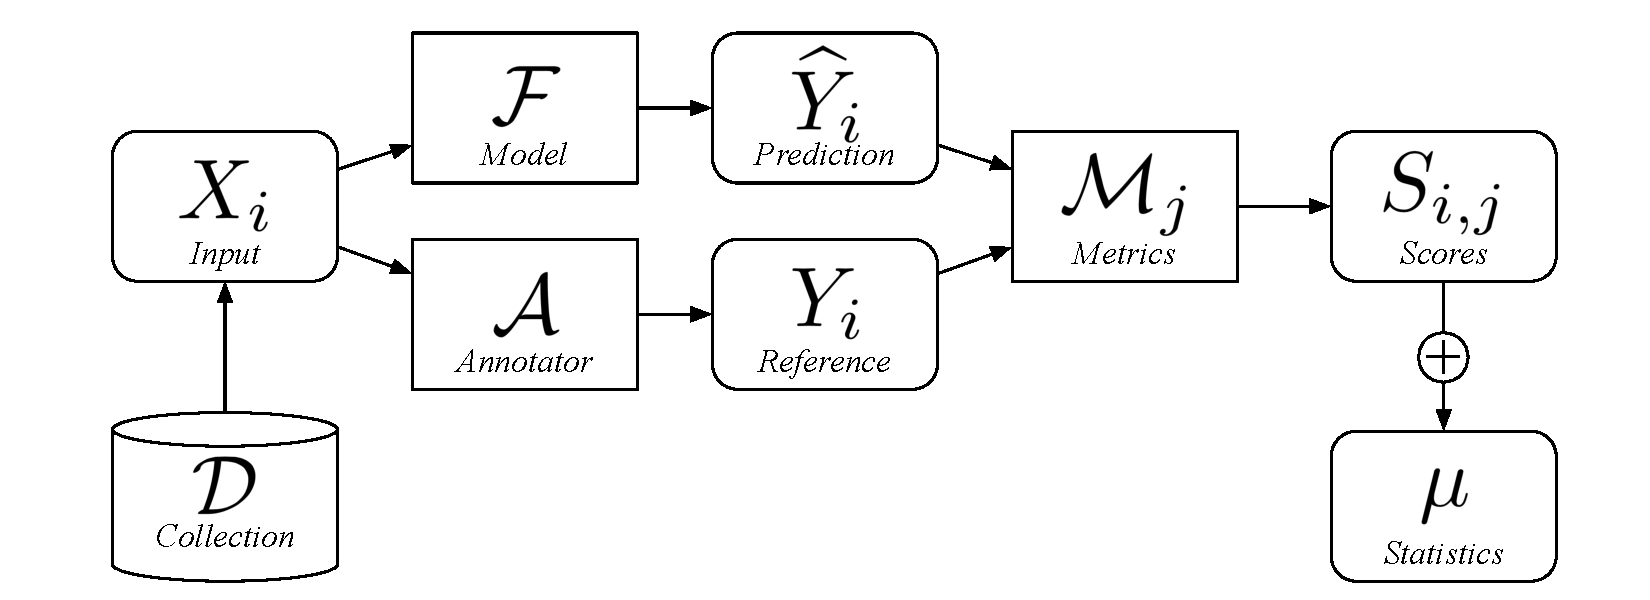
\includegraphics[width=\columnwidth]{eval_framework.pdf}}
 \caption{System diagram of the standard approach to the benchmarking of computational models.}
 \label{fig:system_eval}
\end{figure}

% Transparency and oversight are necessary, this stuff is hard and warrants independent corroboration.
In the current formulation though, a lack of transparency renders participants scientifically blind in a number of ways.
There is no access to any $X_i$, making it impossible to diagnose why an algorithm produced $Z_i$, or determine what should be done to make $\mathcal{F}$ better.
Furthermore, $Y_i$ is meaningless without $X_i$, and must be trivially taken on face value.
By the same token, while $N$ varies from task to task, there is no way to gauge the distribution of the data or how representative it may or may not be.
Limited insight exists into $\mathcal{A}$, the role that subjectivity may play in a given annotation, or the instructions provided when the annotation was initially performed.
As such, the very problem formulation is hidden and subject to drift as it is reinterpreted annually.
For the sake of visibility into $\mathcal{C}^R$, both the original NEMA infrastructure is
open source, and an ongoing community-led effort continues to improve upon these implementations\cite{raffel2014mir_eval}.
And finally, it is only fair to admit that large scale evaluation is a considerable undertaking with plenty of room for error, but conducting these campaigns in the open makes it easier to detect and diagnose any scientific missteps.

% Dearth Data
% MIREX is preoccupied with just keeping the ship afloat.
Somewhat ironically, due to the daunting financial and human costs of the current paradigm, the MIR community, and thus MIREX, suffers from a lack of annotated data.
While this is certainly detrimental to system development, it is absolutely critical to routinely replace the data used for evaluation.
% TODO: soften or justify
Unsurprisingly, in lieu of a fresh source of annotated data, early concerns about the community eventually over-fitting datasets are beginning to manifest.
In some cases, this is because the data used for evaluation exists in the wild, as evidenced by one infamous submission in 2011 that achieved near perfect scores in chord estiamtion having been pretrained on the same data\footnote{http://nema.lis.illinois.edu/nema\_out/mirex2011/results/ace/nmsd2.html}.
% TODO: More detail, converge over multiple iterations.
In others, hidden evaluation data is slowly being over-fit by trial and error, as teams implicitly leverage the weak error signal across campaigns to ``improve'' systems.
These results are misleading due to a fixed, unknown bias in the distribution, which
becomes apparent when datasets are expanded, like the introduction of the Billboard dataset to the chord estimation task in 2012~\cite{burgoyne2011expert}.
% There's no short-term plan to get new data; there's no long-term plan to get new data.
To make matters worse, there is no feasible plan in place to replenish the evaluation datasets currently used by MIREX, never mind a long-term plan to replace that data when it inevitably becomes stale.
By and large, MIREX has relied on the generosity of the community to both curate and donate data for the purposes of evaluation.
This approach also struggles with transparency, making it susceptible to issues of methodology and problem formulation, and can hardly be relied upon as a regular resource.
Data collection is a challenging, unavoidable reality, and one that a demands a viable plan going forward.


\section{Open Evaluation of MIR Systems}

Summarizing the previous section, MIREX suffers from three deficiencies that render the situation terminal:
one, the financial and human cost is far too great to be sustainable indefinitely;
two, limited transparency undermines the scientific value of the endeavor;
and three, the unavoidable, recurring need for freshly annotated data requires a feasible, long-term strategy.


% Here we outline the concrete details of our proposal.
Thus, to address these deficiencies, our proposed plan has three key differentiators from the MIREX model:
\begin{itemize}
\item Distributed computation reduces operating costs to a participant-invariant constant.
\item Using freely available audio facilitates reproducibility.
\item Incremental evaluation encourages that results are scientifically meaningful by
    keeping test data fresh, while steadily increasing the size of datasets available for development and evaluation.
\end{itemize}

% After scores are released from an evaluation campaign, there is still the possibility of long-range over-fit through the feedback loop of score reporting, from which MIREX already suffers.
% To counteract this, different test collections should be introduced each year.
% At first, this seems to get us nowhere: we still need to acquire annotated data, which is presumably expensive.
% We argue that collecting annotations is a better use of resources (both time and funding) than maintaining server execution, as publicly available data benefits many more people than the MIREX participants for any given year.


\subsection{Distributed Computation}
\label{distributed}
The primary difficulty in running an evaluation campaign is computing the outputs of all participating methods.
This difficulty stems from two sources.
First is the obvious computational complexity of running $m$ submissions over $n$ inputs.
Second is the less obvious ``human'' complexity of getting the submitted programs to execute properly in a foreign environment: a task that falls on the small number of task captains each year.
While the computational issues can be ameliorated by executing algorithms in parallel over multiple machines, the cost in human effort has no easy solution in the MIREX framework.

An alternative to this framework is exemplified by Kaggle.\footnote{\url{http://kaggle.com}}
Kaggle competitions are conducted with all input data publicly available, and participants submit only the outputs of their systems, \eg, predictions made for each data point.
This paradigm effectively resolves the difficulties listed above: both computation and manual effort are distributed to the participants, rather than centralized at the evaluation site and task captains.
This dramatically reduces the cost of maintenance and administration.
However, we note a few potential challenges to the distributed computation approach.

First, the test (input) data must be made openly available to participants.
This may increase the risk of bias if participants (unintentionally) tune their algorithms to the evaluation set.
To mitigate bias, we propose the use of a large and diverse corpus of common tracks which are shared across \emph{all tasks}, rather than a collection of small, task-specific datasets as is done in MIREX.
For any given task, only a subset of examples need to be considered when comparing methods, and the evaluation set may be independently selected for each task.
The identity of evaluation sets remains hidden from participants at submission time.
This implies that each submission must span the entire corpus, which reduces the feasibility of participants tuning their algorithms to a specific subset of examples.
Moreover, while this requirement increases computational overhead on the participant's end, it results in a large collection of outputs for various methods on a common corpus, which can be a valuable data source in its own right.

The second challenge is the potential for reduced transparency on behalf of the participants.
While MIREX forces requires submissions to execute on a remote server beyond the participants' control, the scheme proposed here drops that requirement in favor of data transparency.
Consequently, restrictions on the implementation (\eg, running time) would become infeasible, and it may open the possibility of cheating by manual intervention.
Using large test collections with opaque evaluation sets will limit the practicality of
manual participant intervention.%
\footnote{Even in the unlikely event that a participant ``cheats'' by submitting human-generated annotations, the results can be publicly redistributed as free training data, so the community ultimately wins out.}
We argue that trading benefits the community at large, since the availability of open data will serve a broader set of interests over time than the description of methods.

Finally, the proposed scheme assumes that multiple tasks operate on a common input form, \ie, recorded audio.
While the majority of current MIREX tasks do fit into this framework, it precludes tasks requiring symbolic data (score following, symbolic similarity), user interaction (grand challenges, query-by-humming/tapping), or multi-tracks (singing voice separation).


\subsection{Open Content}
\label{open}

For the distributed computation model to be practical, we first need a source of diverse, representative, and freely distributable audio content.
Free audio content is significantly easier to acquire now than when MIREX started, and in particular, a wealth of data can be obtained from Jamendo~\footnote{\url{http://jamendo.com}} and the Free Music Archive (FMA).\footnote{\url{http://freemusicarchive.org/}}
Both of these sites host a variety of music content under either public domain or Creative Commons (CC) licenses.\footnote{\url{https://creativecommons.org/licenses/}}
Since CC-licensed music can be freely redistributed (with attribution), it is (legally) possible to create and share persistent data archives.

The Jamendo and FMA collections are both large and diverse, and both can be linked to meta-data: Jamendo via DBTune to MusicBrainz~\cite{raimond2008web} and FMA to Echo Nest identifiers.
Jamendo claims over 500,000 tracks charted under six major categories: \emph{classical}, \emph{electronic}, \emph{hip-hop}, \emph{jazz}, \emph{pop}, and \emph{rock}.
FMA houses approximately 90,000 tracks which are charted under fifteen categories: \emph{blues}, \emph{classical}, \emph{country}, \emph{electronic}, \emph{experimental}, \emph{folk}, \emph{hip-hop}, \emph{instrumental}, \emph{international}, \emph{jazz}, \emph{old-time/historic}, \emph{pop}, \emph{rock}, \emph{soul/rnb}, and \emph{spoken}.  
These categories should not necessarily be taken as ground truth annotations, but they reflect the tastes and priorities of their respective user communities.
While there is undoubtedly a strong western bias in these corpora, the same is (almost certainly) the case in MIREX's preivate data, but using open content at least permits practitioners to quantify the bias.

This now leads us to the question of representation.
A common criticism of basing research on CC-licensed music is that it is of substantially lower ``quality'' --- which may refer to either artistry or production value, or both --- than commercial music.
This point is obviously valid for high-level tasks such as recommendation, which depend on a variety of factors beyond the raw acoustic content of a track.
However, for the majority of MIREX tasks, in particular the low-level tasks such as beat-tracking or key estimation, this is a much more tenuous case.
We note that FMA includes content by a variety of commercially successful artists,\footnote{\url{https://en.wikipedia.org/wiki/Free\_Music\_Archive#Notable\_artists}} but the vast majority of content in both sources is provided by relatively unknown artists, which makes it difficult to control for ``quality''.

To help users navigate the collections, both Jamendo and FMA provide popularity-based charts and community-based curation services, in addition to the previously mentioned genre categories.
Taken in combination, these indices can be sampled to pre-emptively filter the source collections down to subsets of track which are either of interest to a large number of listeners, of interest to a small number of listeners with specific tastes, or representative of particular styles.
This approach is similar in spirit to previous work using chart-based sampling (typically
Billboard)~\cite{burgoyne2011expert}.

% provide a snapshot torrent for each year's data set
% including for each track:
%   audio
%   metadata (via musicbrainz ids)
%   cc attribution

% what can we say about quality control?
%   maybe do something similar to how MSD was constructed
%       1/3 popular stuff (by play count)
%       1/3 uniform sampling by genre
%       1/3 some random dregs
%   each year, add a sampling of tracks added within the last year

% QC can also happen in evaluation set selection
%   look for disagreements per method
%   when soliciting annotations, allow annotators to flag tracks which are bad for the
%   given task (under an appropriate definition of ``bad'')
%   also solicit confidence ratings in the annotations

%The second point is a difficult one, though FMA does provide some curation.
%It might be interesting to partner with them in helping to guide the selection.

This now leads us to the final point in data collection: which tracks are worth annotating?
Annotating every track for every task would be a monumental undertaking, and an inefficient use of resources.
Several recent studies have investigated the use of algorithm disagreement for detecting ``hard'' examples, be it for beat tracking~\cite{holzapfel2012selective}, structural analysis~\cite[chapter 4]{nieto2015discovering}, or chord recognition~\cite{humphrey2015fourtimely}.
The intuition for this approach is two-fold.
First, tracks for which different algorithms produce significantly different outputs are in some sense ``difficult'' and produce meaningful evaluation results.
Second, if a goal of the evaluation campaign is to differentiate submissions according to some measure of accuracy, then there is little to be gained by spending annotator effort on tracks for which algorithms produce the same output.

%In the proposed framework, we are in a fortunate position of having exactly this type of functionality available to us: participants are submitting system outputs for evaluation!
%It need not be the case that all of the data is being used for evaluation: in fact, Kaggle shows that it is helpful to cloud the space with data that are not included in testing.
%If we are careful about selecting these data, we can then compare the outputs across the participating systems to see which ones are ``interesting'': if the systems generally agree, the example is likely to be easy; at the very least, annotating this track will not help distinguish between these systems.
%If the systems disagree, then we should definitely solicit a strong annotation for the track.
%This is essentially the point made by Urbano et al. %\cite{2012UrbanoXYZ}.

%Each track marked as ``interesting'' should be annotated by at least two humans to determine whether there is actual disagreement.
%It can then be annotated in year 2, and enter the evaluation in year 3.
%By having multiple reference annotations for the ``interesting'' tracks, we can compare algorithm agreement to annotator agreement, and distinguish ``difficult'' tracks from ``ambiguous'' tracks.

%Finally, the fourth point above can be integrated into point 2 by soliciting recommendations from the community.


\subsection{Incremental Evaluation}
% TODO(julian-urbano)


Additionally:

\begin{itemize}
\item Annotation Standards and their enforcement
\item User-facing tools for performing annotations
\item Backend infrastructure for hosting, serving, and collecting submitted annotations (common repository)
\item Would it be possible to leverage citizen science platforms, Mechanical Turk, etc
\end{itemize}


\subsection{Putting it All Together}

Annually, this plan could proceed as follows, as shown in \Cref{fig:cycle}:

First is the \emph{Content Selection} stage.
Here, we provide ``stale'' annotated data --that which shouldn't be used for evaluation any longer-- as training data.
Then, to curate a test set, we combine data previously unseen by the community for which we have annotations, with new, unlabeled content.
This unlabeled content serves to both obscure the datapoints in the test set that \emph{are} annotated, as well as solicit predictions from a large number of automatic algorithms.

Next is the \emph{Competition}, a time-boxed interval spanning a few weeks or months.
Content is made available publicly available is made at the start, such that the training set is provided with labels and the entire test set, without. Some number of submissions are accepted over this internal from registered participants.
A standard format for predictions is defined for each task, and participants can check their submissions against a evaluator to immediately an inkling of how they perform.
This public leaderboard gives insight on some percent of the data. e.g. Kaggle, and at the end of the competition, results are tabulated over the entire holdout set.

After the completion officially closes comes \emph{Incremental Evaluation}. Using the predictions submitted, identify content worth annotating.
It is at this point we can additionally revisit questionable annotations, and perform meta-evalatuation of our common methodology.

Having identified content worthy of investing human effort, the \emph{Annotation} stage proceeds until the next competition.
This is an important distinction, as it takes the most time consuming process --humans describing music-- and largely decouples it as an independent resources.
Thus, annotation spools constantly as a background process, and a snapshot

This virtuous cycle can then repeat indefinitely.
Some particularities are worth mentioning.
For example, it may be necessary to include humans in the evaluation loop at the close of the competition stage, as in user-facing challenges or music similarity ranking.


\section{Discussion}

No free lunch theorem holds.
What follows are a number of topics that have cropped up in the course of writing the paper to date.

\subsection{Human Logistics}

How do we get people to participate / contribute (all jump at once).

At the evaluation level, how do we prevent people from cheating, encourage integrity and the like.
Scale is a good answer for this, but difficult (impossible) to have out of the gate.

We ultimately rely on participants to be honest in their methods and reporting.  What's to prevent a participant from manually annotating all potential test tracks?

I expect that this situation is unlikely.  (However, if people do cheat, we at least get the annotation data, so we still win.)

We may also encourage (require?) participants to release source code to reproduce their methods.  This is in keeping with the spirit of open science and reproducible methods.  I doubt there will be any way to enforce this systematically, but it could be used to audit systems post-hoc.

There's also the matter of selecting which tracks to use in each task.
It may make sense to release a single, large dataset, and require participants to submit annotations for all tracks and for all tasks in which they wish to compete.
If we start getting into the business of slicing down to subsets per task, it will become much easier to determine which tracks are used for which task, and we don't want that.
This all, of course, incurs a greater computational overhead on the participants, but this is A) worth it, from a data collection perspective, and B) how these systems should be used in practice anyway.

We may also consider a two-tiered system, in which closed systems are ranked separately from open systems, which provide voluntary source code.
This may help ease the burden of going fully open source, and encourage submissions from industry.
I think this is a bad idea though.
If it isn't open, it isn't science.
(Just make it cost money then. Which would require the org to NPO-ize).

\subsection{Coverage, or ``What tasks are left out?''}

The system outlined above can apply to any task for which outputs are evaluated by comparing against a reference.
This includes basically everything except for AMS/SMS, where outputs are scored directly.
I argue that these tasks, while interesting, are different enough to fall beyond the scope of the current framework, and may best be left to a separate evaluation campaign.

Alternately, we can treat these left-out tasks as a way to pivot traditional MIREX to focus on things that require direct human evaluation, eg, annual grand challenge tasks.
This way, the MIREX crew gets to keep their current job, and everyone else is happy.

\subsection{Content Validity}

Music is a unique information signal in that its perception is impacted by cultural significance and how this influences expectation and novelty in a listener.
Musical content from the Free Music Archive, or other creative commons sources, are likely to be outside of the gamut of commonly studied music, e.g., popular Western music, and differences in compositional style, instrumentation, or production, may lead to difficulties in validation and generalization.
While this is unlikely to affect tasks such as onset detection or instrument identification, higher level tasks that place greater demand on cognitive aspects of music perception, such as chord estimation or structural analysis, are more sensitive to biased collections.

\subsection{Hosting}

We'll need some infrastructure to actually run the campaign in the new setup.  I think CodaLab might have solved a good chunk of this problem for us.

\subsection{Pay-to-Play}

Ideally, the evaluation data should grow, year upon year, with old data being released to the public either annually or biannually.
To facilitate this, we propose a data credit system.

To participate in an evaluation, each participant must ``pay''� some nominal amount of data credits.
In the first year, all participants start with a balance of 0, so by participating, they are now in ``data debt''�.
Data credits can be earned by providing annotations to be used in the following year's campaign.
A participant is eligible for evaluation in year $X$ when their data credit reaches a non-negative value.

Data credits can be retained across years, and transferred across tasks.

The credits earned can be task-dependent.  Chord annotations might be worth more than beat timings or tempo estimations, for instance.

Data credits may also be earned at a discounted rate by auditing or validating previously provided annotations?  We'll need a system in place to authenticate annotators and force independence.

%Potentially, we may institute a cap-and-trade system to exchange data credits for money which can be used to pay for expert annotations.  Not sure about the legal ramifications of implementing this, or how to organize efforts.  Aside from cash exchange, there might be a benefit to having a task exchange: eg, ``ill trade three beat annotations for one chord annotation�.

\subsection{Next Steps}

To get this off the ground, we'll need a few things:
Evaluation services (already mostly provided by mir\_eval)
An initial seed pool of data (can be inherited from the existing mirex)
A pool of candidate data for evaluation
Infrastructure for managing the exchange
some math / stats to determine how much data we need for each task, each year
some way to work out the data credit rates for different tasks

\section{Misc Refs}
Separate ``labels�'' for systems depending on what they do (eg. close/open, full/subset of dataset): http://trec.nist.gov/pubs/trec22/papers/WEB.OVERVIEW.pdf
Previous proposals (section 8): http://julian-urbano.info/files/publications/051-evaluation-music-information-retrieval.pdf


% For bibtex users:
\bibliography{ISMIRtemplate}

\end{document}
